\documentclass[11pt,a4paper]{article}
\usepackage[utf8]{inputenc}
\usepackage[T1]{fontenc}
\usepackage[spanish,es-tabla]{babel}
\usepackage{lmodern}
\usepackage{geometry}
\geometry{margin=2cm}

\usepackage{amsmath}
\usepackage{amssymb}
\usepackage{siunitx}
\usepackage{graphicx}
\usepackage{xcolor}
\usepackage{tikz}
\usepackage[american, cute inductors, american currents, american voltages]{circuitikz}

\usetikzlibrary{calc, positioning, backgrounds}

\ctikzset{
    logic ports=ieee,
    resistors/scale=0.70,
    capacitors/scale=0.65,
    diodes/scale=0.65,
    transistors/scale=0.80,
    sources/scale=0.70,
    bipoles/thickness=1.0,
    nodes width=0.055
}

\title{\textbf{Proyecto Tatto: Fuente Lineal Regulada}\\
\large Arquitectura Topológica Multinivel y Análisis de Señal}
\author{\textbf{Enjambre de Arquitectura y QA Electrónico}}
\date{\today}

\begin{document}

\maketitle

\begin{abstract}
Este documento presenta el diseño unificado y la síntesis topológica de una Fuente de Alimentación Lineal Regulada de precisión, estructurada en tres niveles jerárquicos de abstracción: Nivel Macro (conversión y potencia), Nivel Silicio (regulador serie con protección de sobrecorriente) y Nivel Transistor (amplificador de error discreto con par diferencial, espejo de corriente, VAS con compensación Miller y driver Push-Pull Clase AB). Asimismo, se incluye la capa analítica de instrumentación virtual superpuesta en tiempo real.
\end{abstract}

\section{Esquemático Maestro Unificado}
El diagrama general multinivel unifica todas las etapas en un solo plano ortogonal sin colisiones espaciales:

\begin{center}
    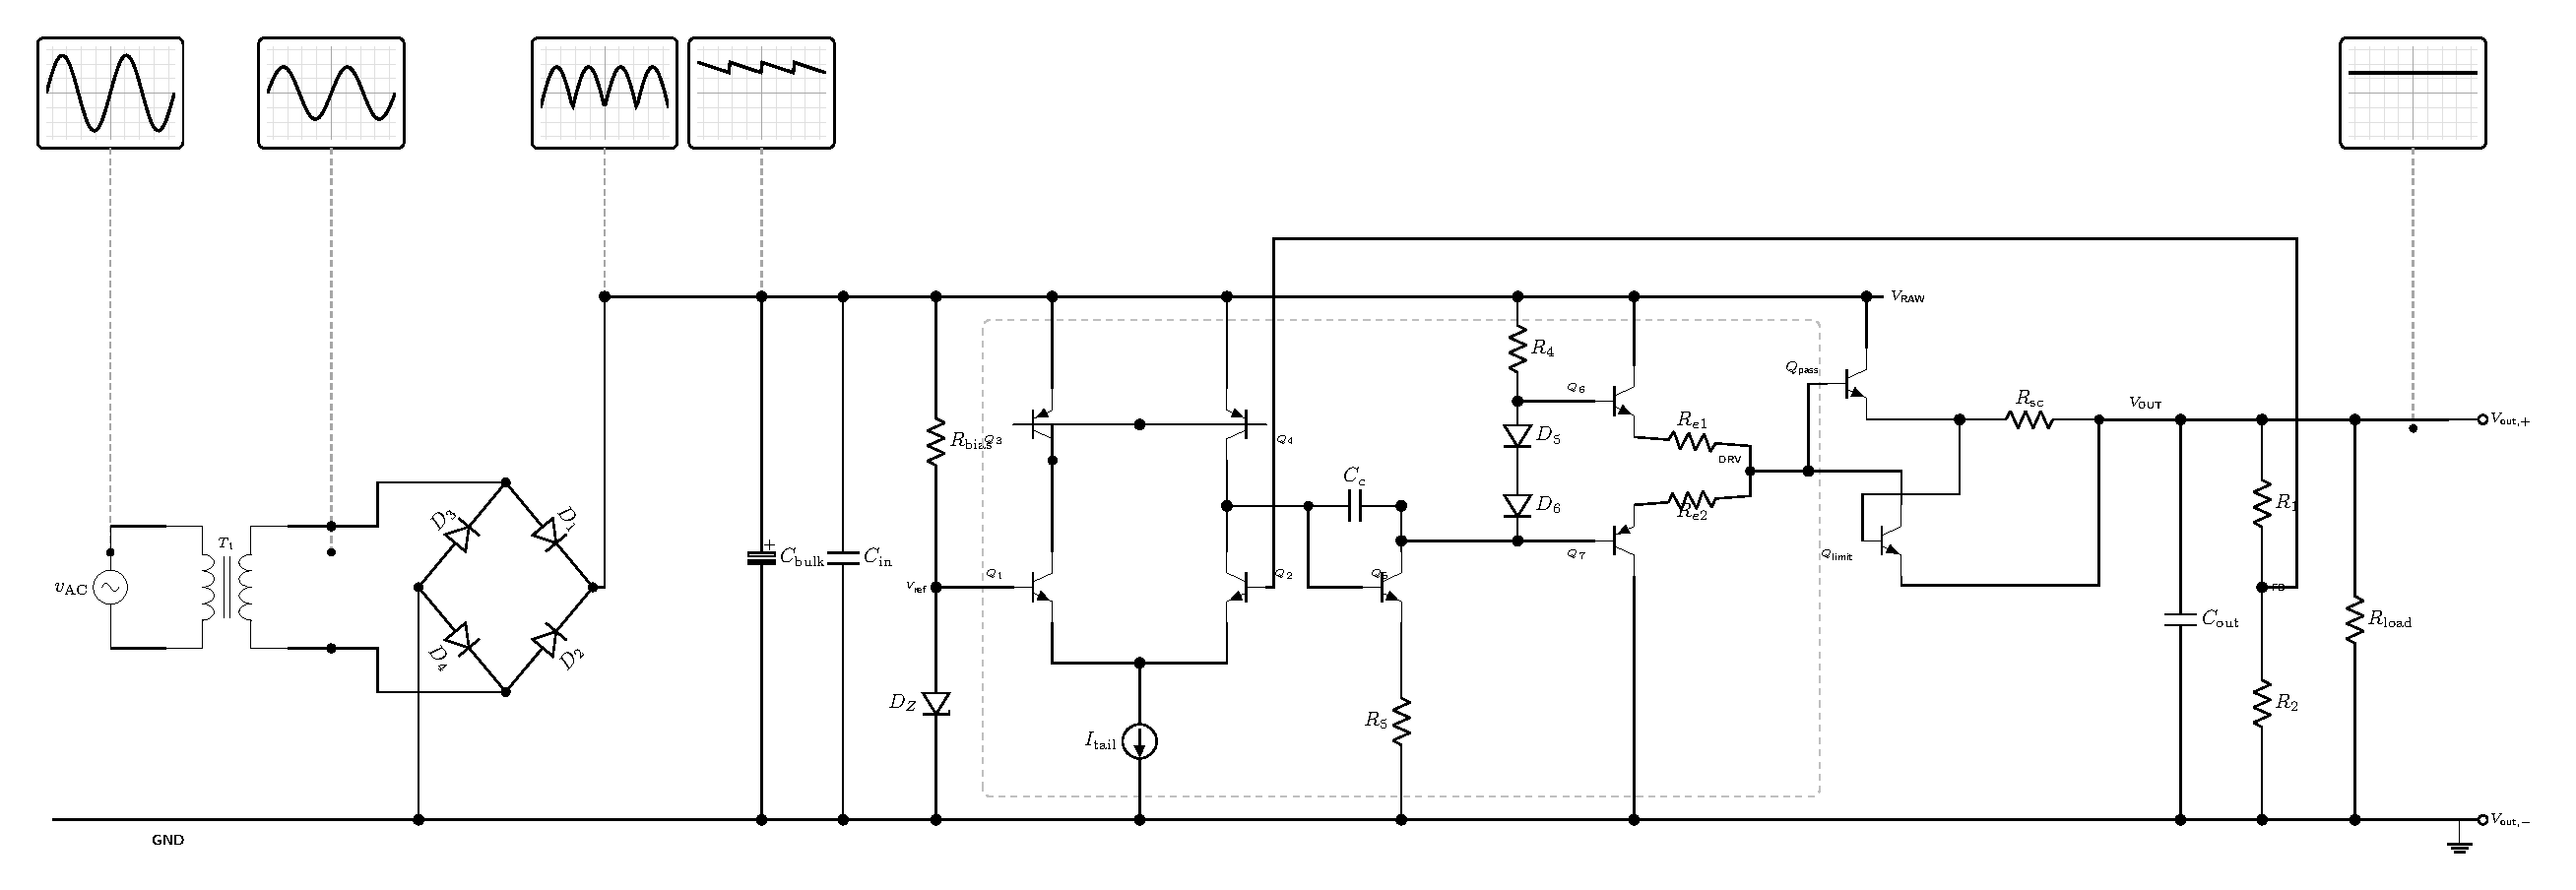
\includegraphics[width=\textwidth]{circuito.pdf}
\end{center}

\section{Sistema de Potencia y Transformación (Nivel Macro)}
\begin{center}
    \begin{circuitikz}[line width=0.75pt, american, scale=0.9, transform shape]
    % Rieles de Potencia
    \draw[line width=1.1pt] (0,0) -- (14.0,0);
    \draw (13.5,0) node[ground] {};
    \node[font=\sffamily\bfseries\scriptsize, below=4pt] at (2.0, 0.0) {$\text{GND}$};
    \draw[line width=1.1pt] (9.5,6.0) -- (14.0,6.0) node[right, font=\sffamily\bfseries\scriptsize] {$V_{\text{RAW}}$};

    % Transformador
    \node[transformer core] (T) at (3.0,3.0) {};
    \node[font=\sffamily\scriptsize\bfseries, below=2pt] at (T.base) {$T_1$};

    % Entrada AC
    \draw (1.0, 0 |- T.A2) to[sV, l=$v_{\text{AC}}$] (1.0, 0 |- T.A1);
    \draw (1.0, 0 |- T.A1) -- (T.A1);
    \draw (1.0, 0 |- T.A2) -- (T.A2);

    % Secundario
    \coordinate (VAC1) at (4.8, 0 |- T.B1);
    \coordinate (VAC2) at (4.8, 0 |- T.B2);
    \draw (T.B1) -- (VAC1) node[circ, fill=black, inner sep=1.2pt] {};
    \draw (T.B2) -- (VAC2) node[circ, fill=black, inner sep=1.2pt] {};

    % Puente en Diamante Planar
    \coordinate (BR_AC1) at (7.8, 4.5);
    \coordinate (BR_AC2) at (7.8, 1.5);
    \coordinate (BR_GND) at (6.3, 3.0);
    \coordinate (BR_VRAW) at (9.3, 3.0);

    \draw (VAC1) -- (5.6, 0 |- VAC1) |- (BR_AC1);
    \draw (VAC2) -- (5.6, 0 |- VAC2) |- (BR_AC2);

    \draw (BR_AC1) to[D, l=$D_1$] (BR_VRAW);
    \draw (BR_AC2) to[D, l_=$D_2$] (BR_VRAW);
    \draw (BR_GND) to[D, l=$D_3$] (BR_AC1);
    \draw (BR_GND) to[D, l_=$D_4$] (BR_AC2);

    \node[circ, fill=black, inner sep=1.2pt] at (BR_AC1) {};
    \node[circ, fill=black, inner sep=1.2pt] at (BR_AC2) {};
    \node[circ, fill=black, inner sep=1.2pt] at (BR_GND) {};
    \node[circ, fill=black, inner sep=1.2pt] at (BR_VRAW) {};

    \draw (BR_GND) -- (6.3, 0.0) node[circ, fill=black, inner sep=1.2pt] {};
    \draw (BR_VRAW) -- (9.5, 3.0) -- (9.5, 6.0) node[circ, fill=black, inner sep=1.2pt] {};

    % Filtro Capacitivo
    \draw (11.5, 6.0) to[eC, l=$C_{\text{bulk}}$, *-*] (11.5, 0.0);
    \draw (13.0, 6.0) to[C, l=$C_{\text{in}}$, *-*] (13.0, 0.0);
\end{circuitikz}

\end{center}

\section{Etapa de Regulación Lineal (Nivel Silicio)}
\begin{center}
    \begin{circuitikz}[line width=0.75pt, american, scale=0.9, transform shape]
    % Rieles
    \draw[line width=1.1pt] (0,0) -- (16.0,0);
    \draw (15.5,0) node[ground] {};
    \node[font=\sffamily\bfseries\scriptsize, below=4pt] at (1.0, 0.0) {$\text{GND}$};
    \draw[line width=1.1pt] (0,7.0) -- (6.0,7.0) node[font=\sffamily\bfseries\scriptsize, above] at (1.0,7.0) {$V_{\text{RAW}}$};

    % Referencia de Voltaje Zener
    \coordinate (VREF) at (2.0, 3.5);
    \draw (2.0, 7.0) to[R, l=$R_{\text{bias}}$, *-*] (VREF);
    \draw (VREF) to[zD, l_=$D_Z$, -*] (2.0, 0.0);
    \node[font=\sffamily\tiny\bfseries, left=1pt] at (VREF) {$V_{\text{ref}}$};

    % Amplificador de Error
    \node[op amp, noinv input up] (OA) at (4.5, 3.0) {};
    \draw (VREF) -- (OA.+);

    % Transistor de Paso de Potencia (Q_pass)
    \node[npn] (Qpass) at (8.0, 5.5) {};
    \node[font=\sffamily\scriptsize\bfseries, above left=1pt] at (Qpass.B) {$Q_{\text{pass}}$};
    \draw (Qpass.C) -- (Qpass.C |- 0, 7.0) node[circ, fill=black, inner sep=1.2pt] {};
    \draw (OA.out) -- (6.0, 3.0) |- (Qpass.B) node[circ, fill=black, inner sep=1.2pt] (NB) {};

    % Sensado de Corriente y Protección (R_sc y Q_limit)
    \coordinate (SENSE) at (9.5, 0 |- Qpass.E);
    \draw (Qpass.E) -- (SENSE) node[circ, fill=black, inner sep=1.2pt] {};

    \coordinate (VOUT_NODE) at (12.0, 0 |- Qpass.E);
    \draw (SENSE) to[R, l=$R_{\text{sc}}$] (VOUT_NODE);
    \node[circ, fill=black, inner sep=1.2pt] at (VOUT_NODE) {};

    \node[npn] (Qlim) at (8.8, 3.5) {};
    \node[font=\sffamily\tiny\bfseries, below left=1pt] at (Qlim.B) {$Q_{\text{limit}}$};

    \draw (SENSE) -- (9.5, 4.2) -| (Qlim.B);
    \draw (Qlim.E) |- (12.0, 2.5) -- (VOUT_NODE);
    \draw (Qlim.C) |- (NB);

    % Riel de Salida
    \draw[line width=1.1pt] (VOUT_NODE) -- (16.0, 0 |- Qpass.E);
    \node[font=\sffamily\bfseries\scriptsize, above=2pt] at (13.0, 0 |- Qpass.E) {$V_{\text{OUT}}$};

    % Divisor de Retroalimentación
    \coordinate (FB_TAP) at (13.5, 2.5);
    \draw (13.5, 0 |- Qpass.E) node[circ, fill=black, inner sep=1.2pt] {} to[R, l=$R_1$] (FB_TAP) node[circ, fill=black, inner sep=1.2pt] {} to[R, l=$R_2$, -*] (13.5, 0.0);
    \node[font=\sffamily\tiny\bfseries, right=1pt] at (FB_TAP) {$\text{FB}$};

    % Retorno de Retroalimentación al Op-Amp
    \draw (FB_TAP) -- (13.5, 1.5) -- (3.0, 1.5) |- (OA.-);

    % Desacoplo y Carga
    \draw (14.8, 0 |- Qpass.E) to[C, l=$C_{\text{out}}$, *-*] (14.8, 0.0);
    \draw (16.0, 0 |- Qpass.E) to[short, -o] (16.5, 0 |- Qpass.E) node[right, font=\sffamily\bfseries\scriptsize] {$V_{\text{out},+}$};
    \draw (16.0, 0.0) to[short, -o] (16.5, 0.0) node[right, font=\sffamily\bfseries\scriptsize] {$V_{\text{out},-}$};
\end{circuitikz}

\end{center}

\section{Amplificador de Error Discreto (Nivel Transistor)}
\begin{center}
    \begin{circuitikz}[line width=0.75pt, american, scale=0.9, transform shape]
    % Rieles de Alimentación
    \draw[line width=1.1pt] (0,0) -- (16.0,0);
    \draw (15.5,0) node[ground] {};
    \node[font=\sffamily\bfseries\scriptsize, below=4pt] at (1.0, 0.0) {$\text{GND}$};
    \draw[line width=1.1pt] (0,8.5) -- (16.0,8.5) node[right, font=\sffamily\bfseries\scriptsize] {$V_{\text{RAW}}$};

    % Entradas
    \draw (0.5, 4.0) node[left, font=\sffamily\scriptsize\bfseries] {$V_{\text{ref}}$} to[short, o-] (2.0, 4.0);
    \draw (0.5, 2.0) node[left, font=\sffamily\scriptsize\bfseries] {$\text{FB}$} to[short, o-] (5.0, 2.0);

    % Par Diferencial de Entrada NPN (Q1, Q2)
    \node[npn] (Q1) at (2.0, 4.0) {};
    \node[npn, xscale=-1] (Q2) at (5.0, 4.0) {};
    \node[font=\sffamily\tiny\bfseries, above left=1pt] at (Q1.B) {$Q_1$};
    \node[font=\sffamily\tiny\bfseries, above right=1pt] at (Q2.B) {$Q_2$};

    % Conexión Emisores a Fuente de Cola
    \coordinate (TAIL) at (3.5, 2.7);
    \draw (Q1.E) |- (TAIL) node[circ, fill=black, inner sep=1.2pt] {} -| (Q2.E);
    \draw (TAIL) to[isource, l_=$I_{\text{tail}}$, -*] (3.5, 0.0);
    \draw (5.0, 2.0) |- (Q2.B);

    % Carga Activa: Espejo de Corriente PNP (Q3, Q4)
    \node[pnp] (Q3) at (2.0, 6.8) {};
    \node[pnp, xscale=-1] (Q4) at (5.0, 6.8) {};
    \node[font=\sffamily\tiny\bfseries, below left=2pt] at (Q3.B) {$Q_3$};
    \node[font=\sffamily\tiny\bfseries, below right=2pt] at (Q4.B) {$Q_4$};

    \draw (Q3.E) -- (Q3.E |- 0, 8.5) node[circ, fill=black, inner sep=1.2pt] {};
    \draw (Q4.E) -- (Q4.E |- 0, 8.5) node[circ, fill=black, inner sep=1.2pt] {};

    \draw (Q1.C) -- (Q3.C);
    \draw (Q2.C) -- (Q4.C) coordinate[midway] (N2);

    \draw (Q3.B) -- (Q4.B);
    \draw (Q3.C) |- (3.5, 6.8) node[circ, fill=black, inner sep=1.2pt] {};
    \node[circ, fill=black, inner sep=1.2pt] at (Q3.C) {};

    % Etapa VAS y Compensación Miller
    \node[npn] (Q5) at (8.0, 4.0) {};
    \node[font=\sffamily\tiny\bfseries, above right=1pt] at (Q5.B) {$Q_5$};

    \coordinate (VAS_IN) at (6.6, 5.4);
    \draw (N2) node[circ, fill=black, inner sep=1.2pt] {} -- (VAS_IN) |- (Q5.B);
    \draw (Q5.E) to[R, l_=$R_5$, -*] (Q5.E |- 0, 0.0);

    % Cadena de Polarización de Drivers
    \coordinate (BIAS_TOP) at (10.0, 7.2);
    \draw (10.0, 8.5) node[circ, fill=black, inner sep=1.2pt] {} to[R, l=$R_4$] (BIAS_TOP) node[circ, fill=black, inner sep=1.2pt] {};

    \coordinate (BIAS_BOT) at (10.0, 4.8);
    \draw (BIAS_TOP) to[D, l=$D_5$] (10.0, 6.0) to[D, l=$D_6$] (BIAS_BOT) node[circ, fill=black, inner sep=1.2pt] {};

    \coordinate (VAS_COL_TAP) at (Q5.C |- 0, 5.4);
    \draw (Q5.C) -- (VAS_COL_TAP) node[circ, fill=black, inner sep=1.2pt] {};
    \draw (Q5.C |- 0, 4.8) node[circ, fill=black, inner sep=1.2pt] {} -- (BIAS_BOT);

    \draw (VAS_COL_TAP) to[C, l_=$C_c$] (VAS_IN);
    \node[circ, fill=black, inner sep=1.2pt] at (VAS_IN) {};

    % Driver Push-Pull Clase AB (Q6, Q7)
    \node[npn] (Q6) at (12.0, 7.2) {};
    \node[pnp] (Q7) at (12.0, 4.8) {};
    \node[font=\sffamily\tiny\bfseries, above left=1pt] at (Q6.B) {$Q_6$};
    \node[font=\sffamily\tiny\bfseries, below left=1pt] at (Q7.B) {$Q_7$};

    \draw (BIAS_TOP) -- (Q6.B);
    \draw (BIAS_BOT) -- (Q7.B);

    \draw (Q6.C) -- (Q6.C |- 0, 8.5) node[circ, fill=black, inner sep=1.2pt] {};
    \draw (Q7.C) -- (Q7.C |- 0, 0.0) node[circ, fill=black, inner sep=1.2pt] {};

    \coordinate (DRV) at (14.0, 6.0);
    \draw (Q6.E) to[R, l=$R_{e1}$] (14.0, 6.43) -- (DRV);
    \draw (Q7.E) to[R, l_=$R_{e2}$] (14.0, 5.57) -- (DRV);
    \node[circ, fill=black, inner sep=1.2pt] at (DRV) {};
    \node[font=\sffamily\tiny\bfseries, above left=1pt] at (DRV) {$\text{DRV}$};
\end{circuitikz}

\end{center}

\end{document}